\newpage % ============================================= Newpage ===================

\begin{figure}[ht]
  \section{Möglichkeiten der Ansteuerung des Druckers}

\adjustbox{valign=t}{\begin{minipage}[t]{0.45\textwidth}
\subsection{RAMPS 1.4}
\begin{framed}
  
\includegraphics[width=1.0\textwidth, trim = 0px 0px 0px 0px, clip]{./bilder/RAMPS14.pdf}
\end{framed}
\end{minipage}}
% \hfill
\adjustbox{valign=t}{\begin{minipage}[t]{0.45\textwidth}
\subsection{SmoothieBoard}
\vspace{-0.34cm}
\begin{framed}
  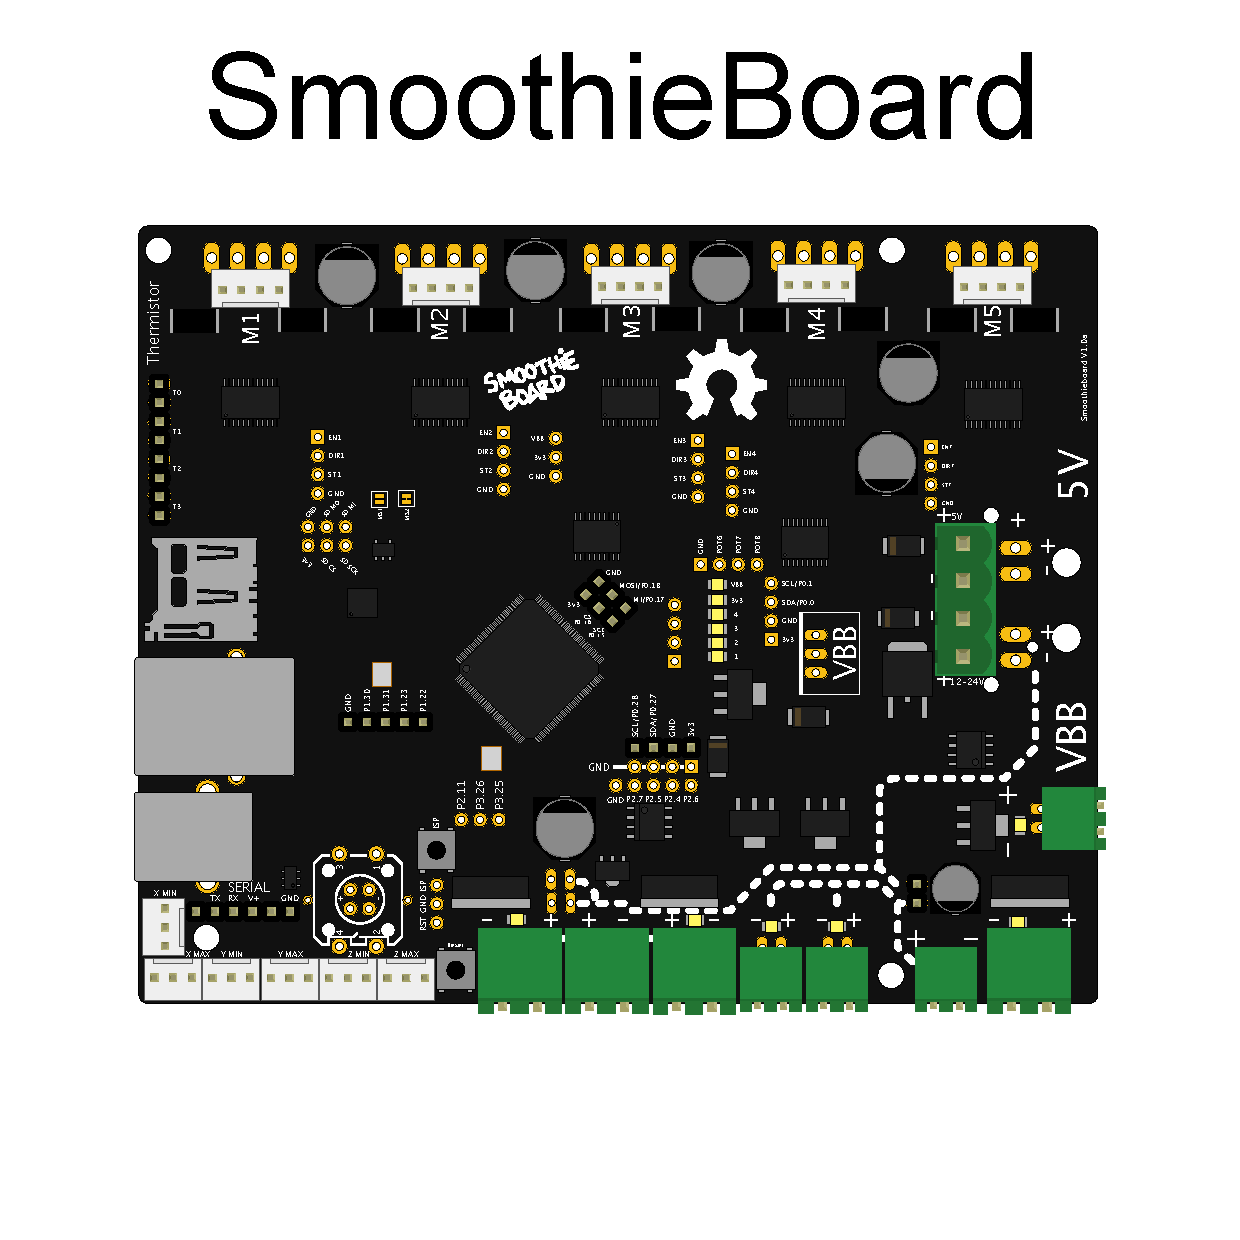
\includegraphics[width=1.0\textwidth, trim = 0px 0px 0px 0px, clip]{./bilder/SmoothieBoard.pdf}
\end{framed}
\end{minipage}}

% \hfill

\adjustbox{valign=t}{\begin{minipage}[t]{0.45\textwidth}
\vspace{0,3cm}
\huge
\textbf{Vorteile}
\begin{itemize}
  \item Extrem Billig \\(inkl. Arduino ca 12€)
  \item Große community
\end{itemize}
% \caption{Kapazität}
\end{minipage}}
% \end{figure}
% \vspace{0.5cm} % ----------------------------------- vspace
% \begin{figure}[ht]
% \hfill
\adjustbox{valign=t}{\begin{minipage}[t]{0.45\textwidth}
\vspace{0,3cm}
\huge
\textbf{Vorteile}
\begin{itemize}
  \item 32 Bit @ 120 MHz, \\ viel Flash und Ram
  \item Ethernet, 4 Temp.-Sensoren
  \item Mit Stepper-Driver bestückt
\end{itemize}

% \caption{Kapazität}
\end{minipage}}
\end{figure}

\clearpage % GleitObjekte anzeigen





\newpage % ============================================= Newpage ===================
% \vspace{-3cm}
\begin{figure}[ht]
  % \section{Möglichkeiten der Ansteuerung des Druckers}

\adjustbox{valign=t}{\begin{minipage}[t]{0.40\textwidth}
% \section{RAMPS 1.4}
\begin{framed}
  
\includegraphics[width=1.0\textwidth, trim = 0px 0px 0px 0px, clip]{./bilder/RAMPS14.pdf}
\end{framed}
\end{minipage}}
% \hfill
\adjustbox{valign=t}{\begin{minipage}[t]{0.40\textwidth}
% \section{SmoothieBoard}
% \vspace{-0.34cm}
\begin{framed}
  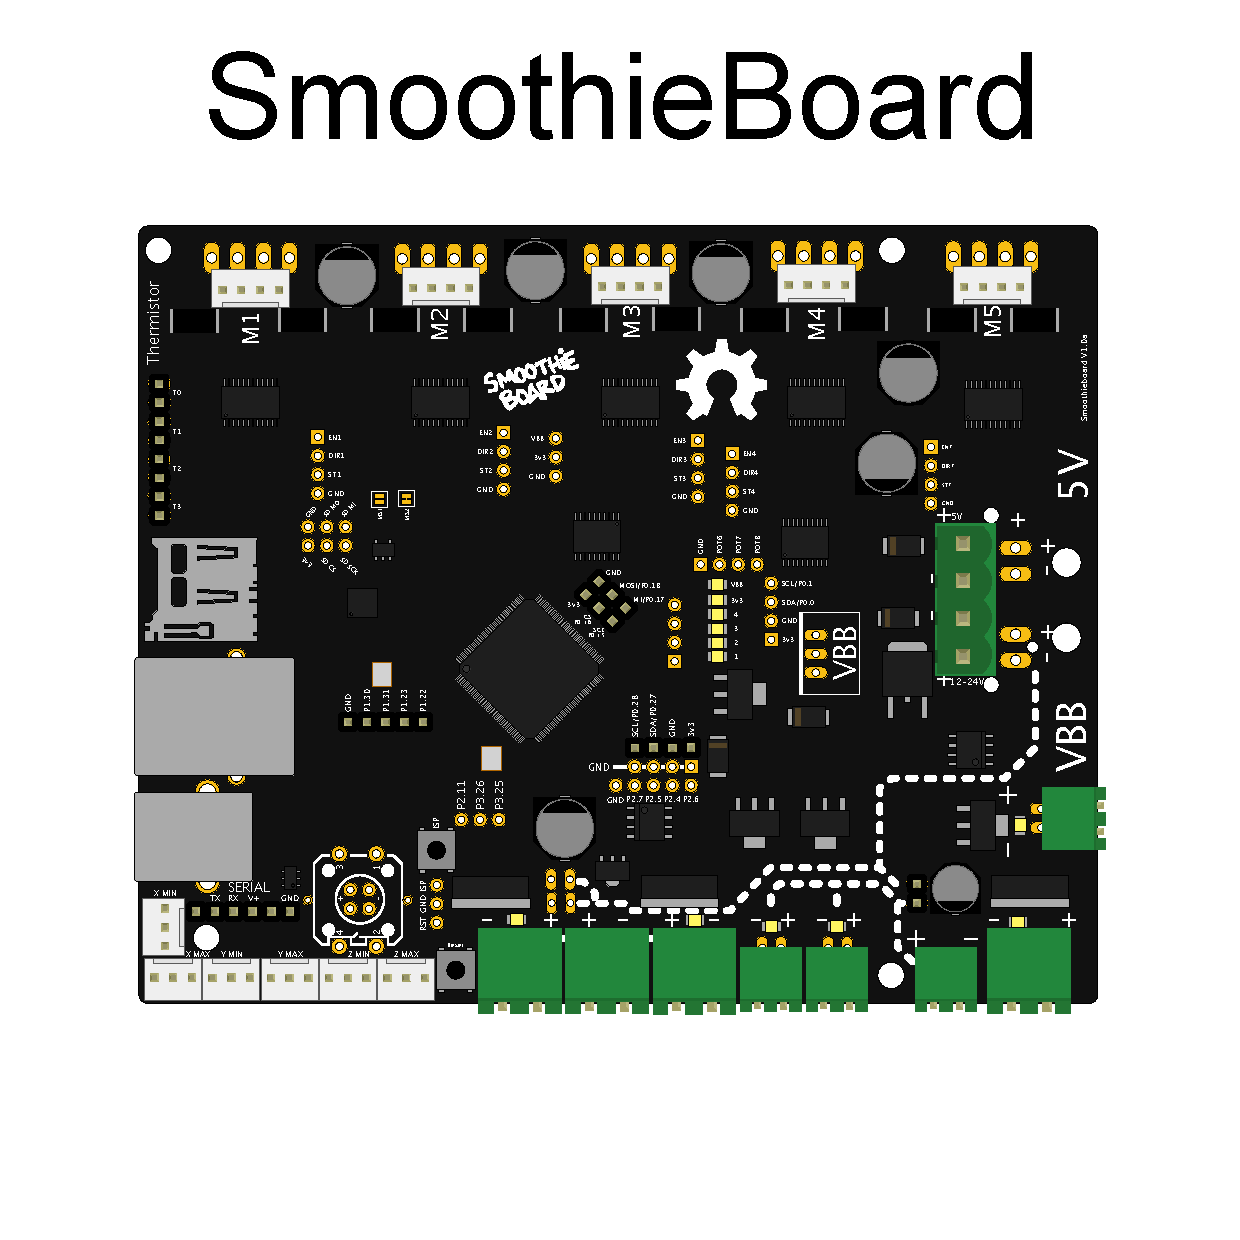
\includegraphics[width=1.0\textwidth, trim = 0px 0px 0px 0px, clip]{./bilder/SmoothieBoard.pdf}
\end{framed}
\end{minipage}}

% \hfill

\adjustbox{valign=t}{\begin{minipage}[t]{0.40\textwidth}
\vspace{0,3cm}
\huge
\textbf{Nachteile}
\begin{itemize}
  \item 8 Bit @ 12 MHZ
  \item Nur EEprom
  \item Wenig Ampere für \\ das Heatbed
  \item Brandgefahr !!! Die \\Stecker sind Schrott.
\end{itemize}
% \caption{Kapazität}
\end{minipage}}
% \end{figure}
% \vspace{0.5cm} % ----------------------------------- vspace
% \begin{figure}[ht]
% \hfill
\adjustbox{valign=t}{\begin{minipage}[t]{0.40\textwidth}
\vspace{0,3cm}
\huge
\textbf{Nachteile}
\begin{itemize}
  \item 32 Bit 120 MHz, \\viel Flash/Ram,
  \item Lan-Anschluss, \\4 Thermal-Sensoren
  \item Mit Stepper-Driver \\bestückt
\end{itemize}

% \caption{Kapazität}
\end{minipage}}
\end{figure}

\clearpage % GleitObjekte anzeigen

% Rampswire14


\newpage % ============================================= Newpage ===================

\begin{figure}[ht]
  % \section{Möglichkeiten der Ansteuerung des Druckers}

  \adjustbox{valign=t}{\begin{minipage}[t]{0.45\textwidth}
  \vspace{0,3cm}
  \huge
  \textbf{Open Hardware}\\
  Beide Boards sind Open Source.\\
  (Alle Abbildung RAMPS)
  % \caption{Kapazität}
  \end{minipage}}
  \hspace{-7cm}
  \adjustbox{valign=t}{\begin{minipage}[t]{0.45\textwidth}
  % \section{SmoothieBoard}
  % \vspace{-0.34cm}
  % \begin{framed}
    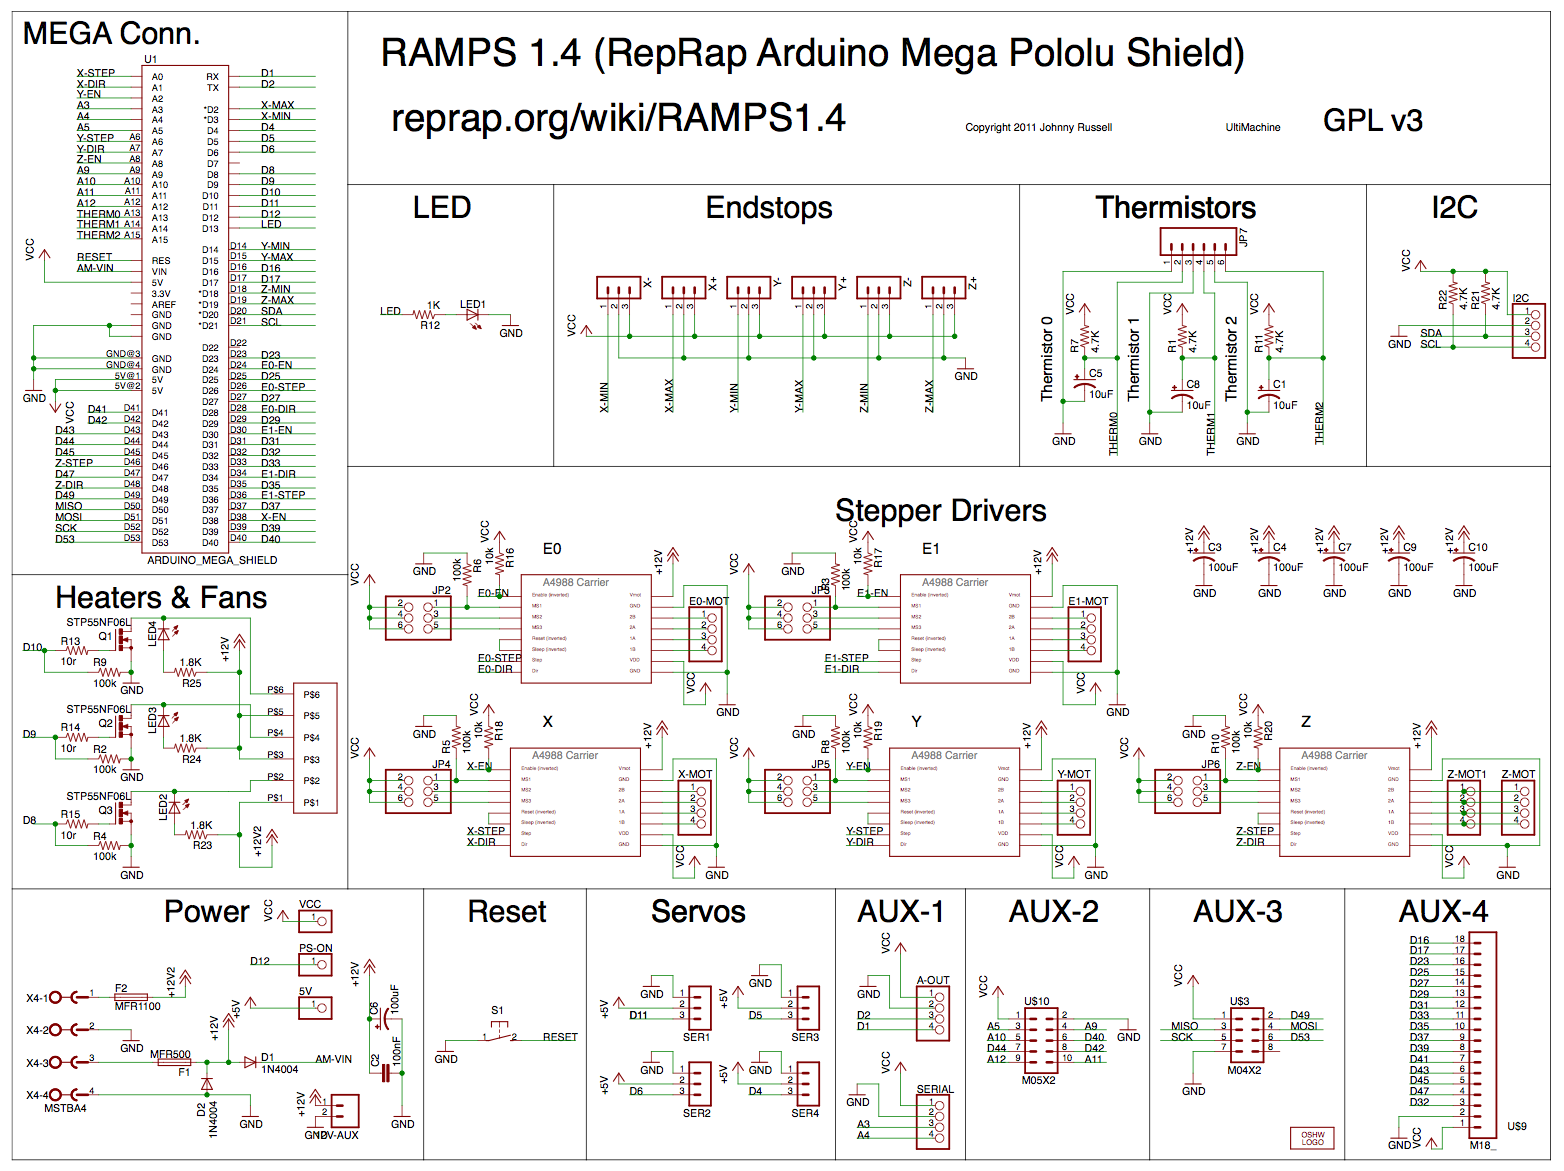
\includegraphics[width=1.0\textwidth, trim = 0px 0px 0px 0px, clip]{./bilder/RAMPS14schematic.png}
  % \end{framed}
  \end{minipage}}
\adjustbox{valign=t}{\begin{minipage}[t]{0.45\textwidth}
% \section{RAMPS 1.4}
\vspace{-4cm}
% \begin{framed}
  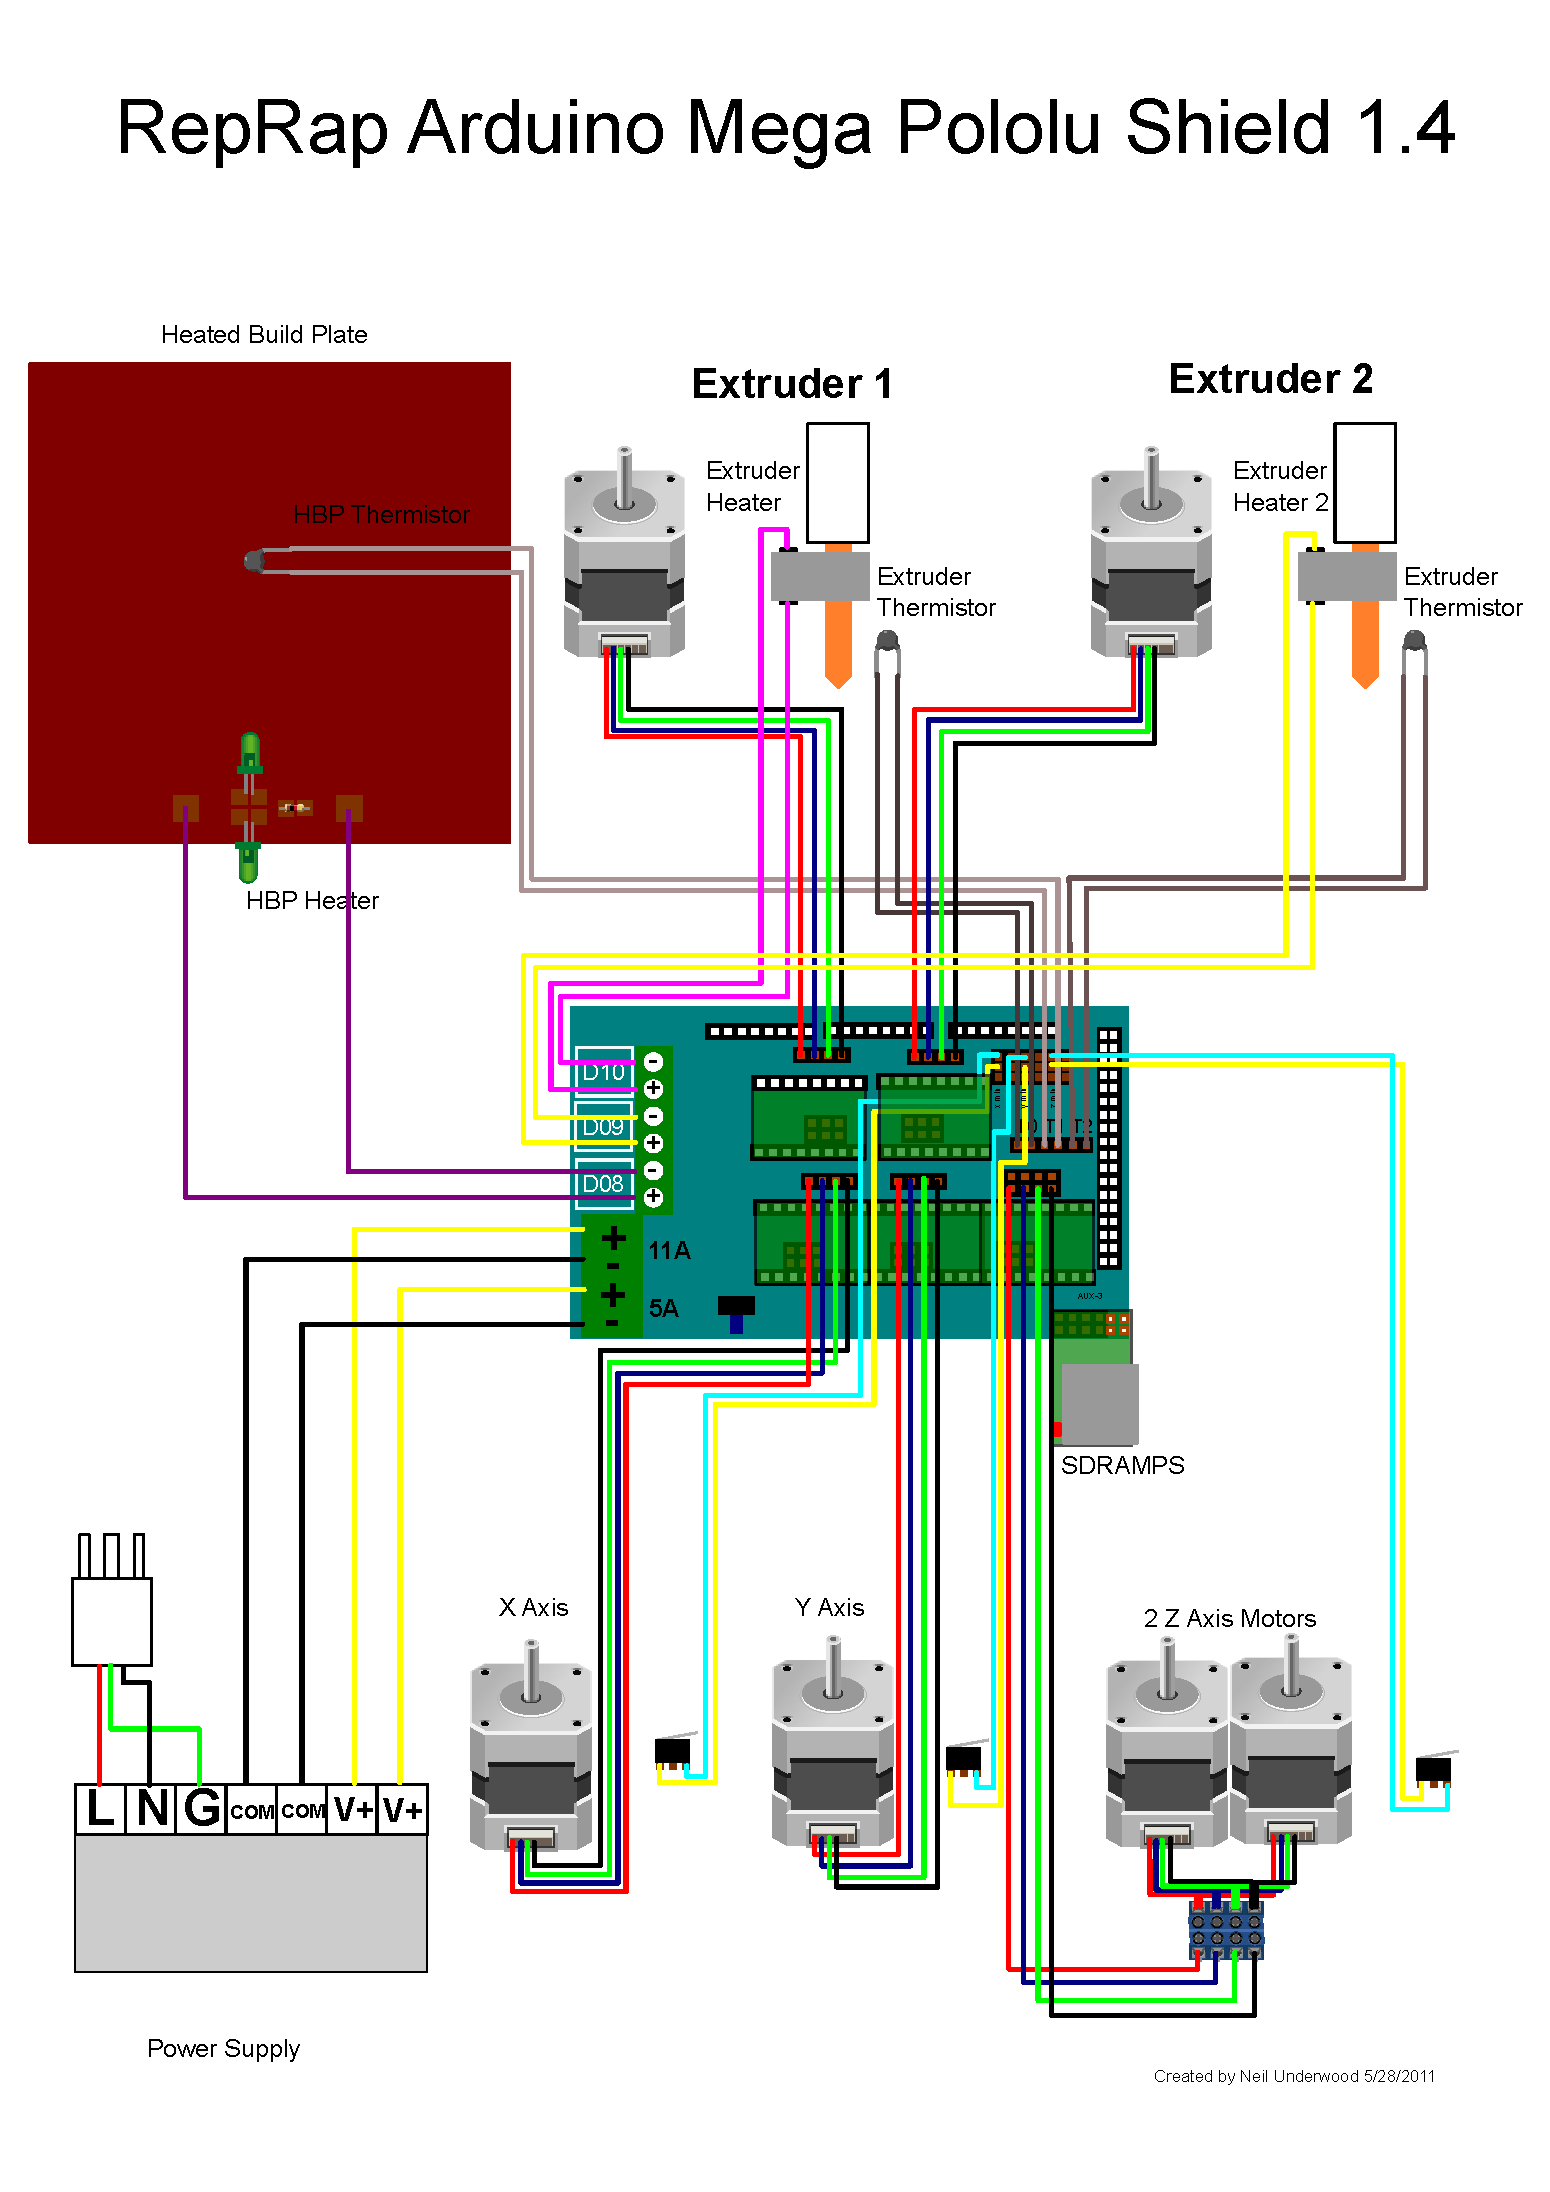
\includegraphics[width=1.0\textwidth, trim = 0px 30px 0px 150px, clip]{./bilder/Rampswire14.pdf}
% \end{framed}
\end{minipage}}
% \hfill
% \hfill
% \end{figure}
% \vspace{0.5cm} % ----------------------------------- vspace
% \begin{figure}[ht]
% \hfill
% ======================================================
\adjustbox{valign=t}{\begin{minipage}[t]{0.45\textwidth}
% \section{SmoothieBoard}
% \vspace{-0.34cm}
% \begin{framed}
  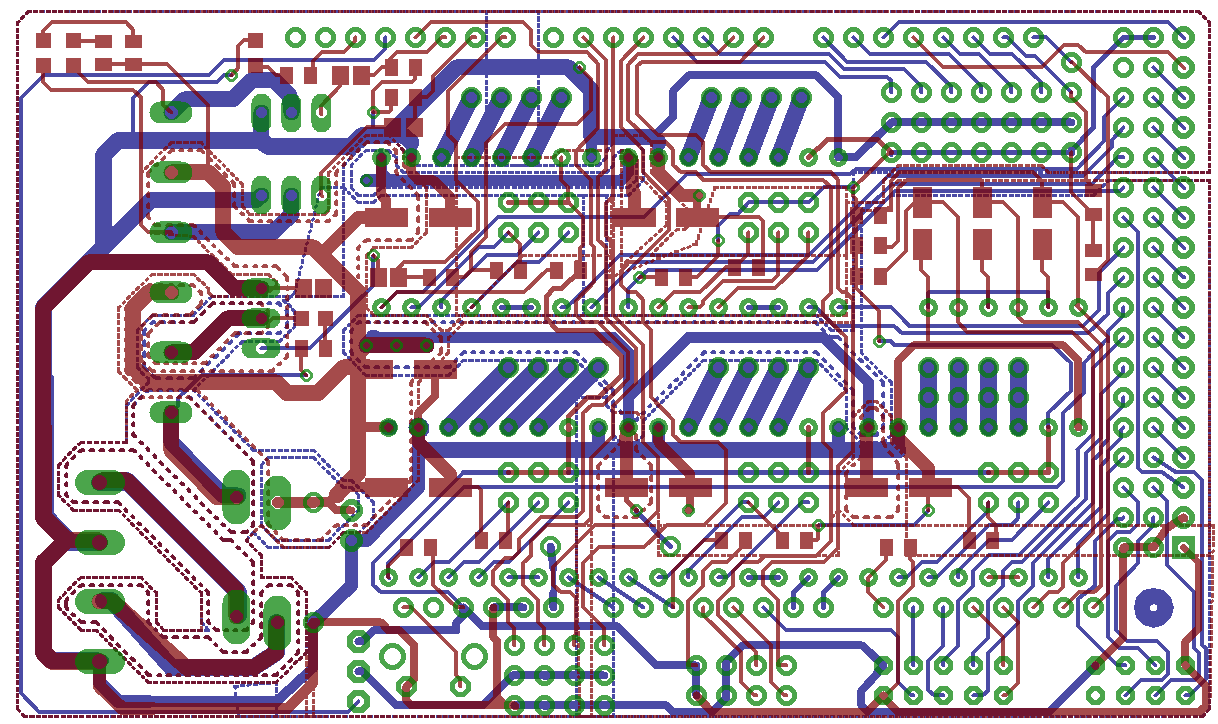
\includegraphics[width=1.0\textwidth, trim = 0px 0px 0px 0px, clip]{./bilder/Ramps14shieldBothsides.png}\\

  Das Smoothieboard ist ähnlich gut Dokumentiert.
% \end{framed}
\end{minipage}}

% ======================================================

% \adjustbox{valign=t}{\begin{minipage}[t]{0.45\textwidth}
% \vspace{0,3cm}
% \huge
% \textbf{Nachteile}
% \begin{itemize}
%   \item 32bit 120 MHz, viel Flash/Ram,
%   \item Lan-Anschluss, 4 Thermal-Sensoren
%   \item Mit Stepper-Driver bestückt
% \end{itemize}
%
% % \caption{Kapazität}
% \end{minipage}}
\end{figure}

\clearpage % GleitObjekte anzeigen

\newpage % ============================================= Newpage ===================
